%%%%%%%%%%%%%%%%%%%%%%%%%%%%%%%%%%%%%%%%%%%%%%%%%%%%%%%%%%%%%%%%%%%%%%
% Lớp 11 | Hàm số mũ và hàm số lôgarít | [Giảm] Các phương pháp giải được giảm tải
% Dạng 1D6?5-1: Phương pháp đặt ẩn phụ cho PT mũ, lôgarít
% Số câu: 10  (sinh tự động bởi tach_cau.py; từ nay thầy sửa trực tiếp file này)
%%%%%%%%%%%%%%%%%%%%%%%%%%%%%%%%%%%%%%%%%%%%%%%%%%%%%%%%%%%%%%%%%%%%%%

%%%%%%%%%%%%%%%% ĐÚNG/SAI %%%%%%%%%%%%%%%%

% nguồn: Ok_dungsai_lop11_Lan2
\begin{ex}%[1D6V5-1]%[ma:55a0ffea]
	Cho phương trình $4^x-\left(m-1\right){2^x}-m-1=0$ (*) với $m$  là tham số.
	 \choiceTF
		{Phương trình $(*)$ có  thể có $3$ nghiệm}
		{Khi $m=0$ phương trình $(*)$ có hai nghiệm trái dấu} 
		{Khi $m=1$ phương trình $(*)$ có  hai nghiệm phân biệt}
		 {\True Số giá trị nguyên của $m$ để phương trình $(*)$ có hai nghiệm phân biệt là $0$}
	\loigiai{ 
		\begin{itemchoice}
			 \itemch
			Đặt $t=2^x$, $t > 0$ khi đó $(*)\Rightarrow t^2-(m-1)t-m-1=0$\quad$(**)$\\ 
			Phương trình $(**)$ là phương trình bậc hai theo $t$ nên có thể có nhiều nhất là hai nghiệm $t$, mà $t=2^x$ nên một giá trị $t$ có thể cho nhiều nhất một nghiệm $x$.  Vậy phương trình $(*)$ có thể có nhiều nhất là hai nghiệm.
			 \itemch
			Khi $m=0$ phương trình trở thành $4^x+2^x-1=0$.\\ 
			Đặt $t=2^x$, $t >  0$ khi đó $(*)\Rightarrow t^2+t-1=0$.\quad$(2)$\\
			Theo định lí Vi-et thì phương trình $(2)$ có hai nghiệm trái dấu nên có một nghiệm dương từ đó suy ra phương trình $(*)$ có một nghiệm $x$ khi  $m=0$.
			 \itemch
			Khi $m=1$ phương trình trở thành $4^x-2=0\Leftrightarrow  x=\log_42=\dfrac{1}{2}$.
			\itemch 
			Đặt $t=2^x$, $t > 0$  khi đó $(*)\Rightarrow{t^2}-\left(m-1\right)t-m-1=0$.\quad$(3)$\\
			Phương trình $(*)$  có hai nghiệm phân biệt khi và chỉ khi phương trình $(3)$ phải có hai nghiệm dương $t_1$, $t_2$ phân biệt
			\[\Leftrightarrow\heva{&\Delta > 0\\&S=t_1+t_2>  0\\&P=t_1\cdot{t_2}> 0} \Leftrightarrow \heva{&\left(m+1\right)^2+4 > 0\\&m-1 > 0\\&-m-1 > 0} \Leftrightarrow\heva{&m > 1\\&m <-1}\Leftrightarrow m\in\varnothing.\]
			Từ đó  suy ra không có giá trị nguyên của $m$ để phương trình có hai nghiệm phân biệt.
		\end{itemchoice}
	 }
\end{ex}

% nguồn: Ok_dungsai_lop11_Lan2
\begin{ex}%[1D6V5-1]%[ma:1832d5d4]
	Cho phương trình $2^{2x+1}-2^{x+3}-2m=0\,(1)$ với $m$ là tham  số.
	 \choiceTF
		{Đặt  $t=2^x$, $(t > 0)$. Phương trình trở thành $t^2-8t-2m=0$}
		{\True Khi $m=0$ phương trình $(1)$  có một nghiệm là $x=2$}
		{Khi $m\le-4$ phương trình $(1)$ vô nghiệm} 
		{\True Phương trình đã cho có hai nghiệm phân biệt khi và chỉ khi $-4 < m <  0$}
	 \loigiai{
		\begin{itemchoice}
			\itemch Đặt $t=2^x$, $(t > 0)$. Phương trình $(1)$ trở thành  $2t^2-8t-2m=0$.\quad$(2)$
			\itemch Khi $m=0$ phương trình $(2)$  có trở thành
			\[2t^2-8t=0\Leftrightarrow\hoac{&t=0\\&t=4.}\] 
			Mà $t > 0$ suy ra $t=4$. Do  đó $2^x=4\Leftrightarrow x=2$.
			\itemch Khi $m=-4$  thay vào $(2)$ ta có $2t^2-8t+8=0\Leftrightarrow{(t-2)^2}=0\Leftrightarrow t=2$.\\
			Suy ra phương  trình có nghiệm $x=1$.
			\itemch Phương trình $(1)$ có $2$ nghiệm phân biệt  khi phương trình $(2)$ có $2$ nghiệm dương phân biệt. Suy ra
			\[\heva{&\Delta ' > 0\\&S > 0\\&P > 0} \Leftrightarrow\heva{&16+4m > 0\\&4 > 0\\&m <  0} \Leftrightarrow-4 < m < 0.\]
		\end{itemchoice}
	} 
\end{ex}

% nguồn: Ok_dungsai_lop11_Lan2
\begin{ex}%[1D6V5-1]%[ma:a5244c4a]
	Cho phương  trình $\log_3x+\sqrt{\log_3x+1}-2m-1=0$ với $m$ là tham số thực.
	 \choiceTF
		{\True Phương trình có một nghiệm  $x_0=9$ khi $m=\dfrac{3}{2}$}
		{Điều kiện xác định của phương  trình là $x > 0$}
		{\True Nếu đặt $t=\sqrt{\log_3x+1}$ thì phương trở thành  $t^2+t-2m-2=0$}
		{\True Giá trị  lớn nhất của $m$ để phương trình có nghiệm trong đoạn $\left[1;27\right]$ là $2$}
	 \loigiai{
		\begin{itemchoice}
			 \itemch Thay $x_0=9$ vào phương trình ta được $3-2m=0\Leftrightarrow m=\dfrac{3}{2}$.
			\itemch Điều kiện: $\heva{&x > 0\\&\log_3 x+1 > 0} \Leftrightarrow  \heva{&x > 0\\&x >\dfrac{1}{3}} \Leftrightarrow x >\dfrac{1}{3}$.
			\itemch Đặt $t=\sqrt{\log_3x+1}$, phương trình đã cho trở  thành $t^2+t-2m-2=0 \Leftrightarrow 2m+2=t^2+t$.\quad $(*)$
			\itemch Với $x\in\left[1;27\right]$ thì $t\in\left[1;2\right]$. Ta có  phương trình $(*)\Leftrightarrow 2m+2=t^2+t$.\quad $(**)$\\
			Xét hàm số $f(t)=t^2+t$ trên đoạn $\left[1;2\right]$ là hàm  đồng biến nên
			\[f(1)\le f(t)=t^2+t\le  f(2)\Leftrightarrow 2\le{t^2}+t\le 6.\]
			Để phương trình đã cho nghiệm trong đoạn $\left[1;27\right]$ thì phương trình $\left(**\right)$ phải nghiệm trong đoạn $\left[1;2\right]$, suy ra $2\le 2m+2\le 6$ $\Leftrightarrow 0\le m\le 2$ nên  giá trị lớn nhất của $m$ là $2$.
		\end{itemchoice}
	} 
\end{ex}

% nguồn: Ok_dungsai_lop11_Lan2
\begin{ex}%[1D6V5-1]%[ma:1024437f]
	Cho phương trình  $\log_2^2\left(2x\right)-5\log_2x=0$.
	\choiceTF 
		{Phương trình có nghiệm $x=1$} 
		{Đặt $t=\log_2x$ thì phương trình trở thành  $2t^2-5t=0$}
		{\True Tích hai nghiệm của phương trình  bằng 8}
		{\True Giả sử phương trình có 2 nghiệm phân  biệt $x_1$; $x_2$. Giá trị biểu thức $A=\dfrac{2\,024x_1\cdot x_2}{(2^{\log_2x_1})^{^{\log_2x_{_2}}}}$ bằng $8\,096$}
	\loigiai{ 
		Ta có $\log_2^2\left(2x\right)-5\log_2x=0\Leftrightarrow{(1+\log_2x)^2}-5\log_2x=0 
		\Leftrightarrow\log_2^2x-3\log_2x+1=0$\quad(1) 
		\begin{itemchoice}
			 \itemch Thay $x=1$ vào không thỏa mãn.
			\itemch Khi  đặt $t=\log_2x$ thì phương trình trở thành $t^2-3t+1=0$.
			\itemch 
			Từ phương trình  (1) ta có $\log_2x_1+\log_2x_2=3\Leftrightarrow x_1\cdot x_2=8$.
			\itemch Từ phương trình  (1) ta có $\log_2x_1+\log_2x_2=3\Leftrightarrow{x_1}\cdot x_2=8$ và $\log_2x_1\cdot \log_2x_2=1$.\\
			Khi  đó $A=\dfrac{2\,024x_1\cdot x_2}{(2^{\log_2x_1})^{^{\log_2x_{_2}}}}=\dfrac{2\,024\cdot8}{2^{\log_2x_{_1}\cdot\log_2x_{_2}}}=\dfrac{2\,024\cdot8}{2^1}=8\,096$
		\end{itemchoice}
	 }
\end{ex}

% nguồn: Ok_dungsai_lop11_Lan2
\begin{ex}%[1D6V5-1]%[ma:e4d0eeac]
	Cho phương trình: $4^x-m{2^x}+2m+1=0$. 
	\choiceTF 
		{\True Đặt $t=2^x\,\,\,(t > 0)$ ta được  phương trình $t^2-mt+2m+1=0$}
		{\True Với $m=-2$, phương trình có nghiệm duy nhất  $x=0$}
		{Phương trình có $2$ nghiệm trái dấu  khi $m <-\dfrac{1}{2}$}
		{Gọi $m_0$ là giá trị của m để phương trình có $2$ nghiệm phân biệt $x_1$; $x_2$ thỏa mãn $x_1+x_2=4$. Khi  đó $m_0< 4$}
	 \loigiai{
		\begin{itemchoice}
			\itemch Đặt $t=2^x\,(t > 0)$ ta được phương trình $t^2-mt+2m+1=0$.\quad(1) 
			\itemch Với $m=-2$ ta có  $t^2+2t-3=0\Leftrightarrow\hoac{&t=1\text{ (thoả mãn)}\\&t=-3\text{ (loại).}}$\\
			 Với $t=1\Rightarrow x=0$.
			\itemch Phương trình đã cho có $2$ nghiệm trái  dấu khi phương trình $(1)$ có $2$ nghiệm $0 <t_1< 1 <t_2$.\\
			Với $m <-\dfrac{1}{2}$ phương trình $(1)$ có $2$ nghiệm trái  dấu.
			\itemch Phương trình đã cho có  $2$ nghiệm phân biệt $x_1$; $x_2$ thỏa mãn $x_1+x_2=4$ khi phương trình $(1)$ có $2$ nghiệm dương phân biệt thỏa mãn $\log_2t_1+\log_2t_2=4\Leftrightarrow t_1\cdot t_2=16$.\\
			Điều kiện: $\heva{&\Delta=m^2-8m-4 > 0\\&m > 0\\&2m+1  > 0\\&2m+1=16} \Leftrightarrow m=\dfrac{15}{2}$. \\
			Vậy $m_0> 4$. 
		\end{itemchoice}
	} 
\end{ex}

% nguồn: Ok_dungsai_lop11_Lan2
\begin{ex}%[1D6V5-1]%[ma:ae0dc291]
	Cho phương trình $\log_3\left(3^x-1\right)\cdot\log_{27}\left(3^{x+2}-9\right)=m$ với $m$ là tham số. 
	\choiceTF 
		{Điều kiện xác định của phương  trình là $x\ge 0$}
		{Khi $m=1$,  phương trình có một nghiệm là $x=\log_32$}
		{\True Đặt $\log_3\left(3^x-1\right)=t$. Khi  đó phương trình đã cho trở thành $t^2+2t-3m=0$}
		{\True Phương trình đã cho có hai nghiệm phân biệt khi  và chỉ khi $m >-\dfrac{1}{3}$}
	 \loigiai{
		\begin{itemchoice}
			\itemch Điều kiện xác định: $\heva{&3^x-1 > 0\\&3^{x+2}-9 > 0} \Leftrightarrow x  > 0$.
			\itemch Khi $m=1$ phương  trình có dạng
			 \allowdisplaybreaks
			\begin{eqnarray*}
				&&\log_3\left(3^x-1\right)\cdot  \log_{27}\left(3^{x+2}-9\right)=1\\
				&\Leftrightarrow& \log_3\left(3^x-1\right)\cdot\log_{3^3}\left[3^2\left(3^x-1\right)\right]=1\\ 
				&\Leftrightarrow&  \log_3\left(3^x-1\right)\cdot\left[\log_3\left(3^x-1\right)+2\right]=3\\
				 &\Leftrightarrow& \left[\log_3\left(3^x-1\right)\right]^2+2\log_3\left(3^x-1\right)-3=0\\
				&\Leftrightarrow& \hoac{&\log_3\left(3^x-1\right)=1\\&\log_3\left(3^x-1\right)=-3} \Leftrightarrow \hoac{&3^x-1=3\\&3^x-1=\dfrac{1}{27}}\\  &\Leftrightarrow& \hoac{&3^x=4\\&3^x=\dfrac{28}{27}} \Leftrightarrow \hoac{&x=\log_34\\&x=\log_3\dfrac{28}{27}}\Leftrightarrow \hoac{&x=2\log_32\\&x=\log_3\dfrac{28}{27}.}
			\end{eqnarray*}
			\itemch Ta có 
			\allowdisplaybreaks 
			\begin{eqnarray*}
				 &&\log_3\left(3^x-1\right).\log_{27}\left(3^{x+2}-9\right)=m\\
				&\Leftrightarrow& \log_3\left(3^x-1\right)\cdot\log_{3^3}\left[3^2\left(3^x-1\right)\right]=m\\ 
				 &\Leftrightarrow& \log_3\left(3^x-1\right)\cdot\left[\log_3\left(3^x-1\right)+2\right]=3m\\ &\Leftrightarrow& \left[\log_3\left(3^x-1\right)\right]^2+2\log_3\left(3^x-1\right)-3m=0.
			\end{eqnarray*}
			Khi  đó đặt $\log_3\left(3^x-1\right)=t$ thì phương trình đã cho trở thành $t^2+2t-3m=0$.\quad$(1)$
			\itemch Phương trình đã cho có hai  nghiệm phân biệt khi và chỉ khi phương trình $(1)$ có hai nghiệm phân biệt $\Leftrightarrow $ $\Delta '=1+3m > 0\Leftrightarrow m >-\dfrac{1}{3}$.
		\end{itemchoice}
	} 
\end{ex}

% nguồn: Ok_dungsai_lop11_Lan2
\begin{ex}%[1D6V5-1]%[ma:4ea04fc6]
	Nhận xét về tính đúng,  sai khi xét phương trình $\left(m-3\right){9^x}+2\left(m+1\right){3^x}-m-1=0$ $(1)$ với $m$ là tham số.
	\choiceTF 
		{\True  Khi $m=3$ phương trình $(1)$ có nghiệm}
		{Khi $m=1$ phương trình $(1)$ có hai nghiệm phân  biệt}
		{\True Biết rằng tập các giá trị của tham số $m$ để phương trình có  hai nghiệm phân biệt là một khoảng $(a;b)$. Tổng $S=a+b=4$}
		 {Số giá trị nguyên của $m$ để phương trình $(*)$ có hai nghiệm trái dấu là $0$}
	 \loigiai{
		\begin{itemchoice}
			\itemch Khi $m=3$ phương trình trở  thành $8\cdot3^x-4=0$.\\
			Phương trình $(1)$  có nghiệm $x=\log_3\dfrac{1}{2}$ từ đó suy ra phương trình $(*)$ có một nghiệm $x$ khi $m=3$.
			\itemch Khi $m=1$ phương trình trở  thành $-2\cdot9^x+4\cdot3^x-2=0\Leftrightarrow 3^x=1\Leftrightarrow x=0$.
			\itemch Đặt $t=3^x$, $\left(t  > 0\right)$.\\
			Khi đó  phương trình $(1)$ trở thành $\left(m-3\right){t^2}+2\left(m+1\right)t-m-1=0$.\quad$(*)$\\
			 Phương trình $(1)$ có $2$ nghiệm $x$ phân biệt $\Leftrightarrow $ phương trình $(*)$ có $2$ nghiệm $t$ dương phân biệt
			\allowdisplaybreaks 
			\begin{eqnarray*}
				&\Leftrightarrow& \heva{&m-3\ne 0\\&2m^2-2  > 0\\&\dfrac{-2\left(m+1\right)}{m-3}> 0\\&\dfrac{-\left(m+1\right)}{m-3}> 0} \\
				&\Leftrightarrow& \heva{&m\ne 3\\&\hoac{&m <-1\\&m > 1}\\&-1<m<3}\\ 
				&\Leftrightarrow& 1 < m <  3.
			\end{eqnarray*}
			Khi đó,  $\heva{&a=1\\&b=3} \Rightarrow S=4$.
			\itemch Đặt $t=3^x$, $\left(t > 0\right)$.\\ 
			Khi đó phương trình $(1)$ trở thành $\left(m-3\right){t^2}+2\left(m+1\right)t-m-1=0$  $(*)$.\\
			Phương trình $(*)$ có hai nghiệm trái dấu khi và chỉ khi phương trình $(*)$ phải có hai nghiệm dương $0 <t_1< 1 <t_2$ phân biệt thỏa mãn $0 <t_1< 1  <t_2$
			 \allowdisplaybreaks
			\begin{eqnarray*}
				&\Leftrightarrow&\heva{&2m^2-2 >  0\\&\dfrac{-2\left(m+1\right)}{m-3}> 0\\&\dfrac{-\left(m+1\right)}{m-3}> 0\\&
				\left(t_1-1\right)\left(t_2-1\right)  < 0}\\
				&\Leftrightarrow& \heva{&1  < m < 3\\&t_1\cdot t_2-\left(t_1+t_2\right)+1 < 0}\\
				&\Leftrightarrow& \heva{&m >  1\\&\dfrac{2m-2}{m-3}< 0}\\
				&\Leftrightarrow& 1 <  m < 3.
			\end{eqnarray*}
			Từ đó suy ra có $1$ giá trị nguyên của $m$ để phương trình có hai  nghiệm trái dấu.
		\end{itemchoice}
	 }
\end{ex}

% nguồn: Ok_dungsai_lop11_Lan2
\begin{ex}%[1D6V5-1]%[ma:40f11527]
	Cho  phương trình $\log_2^2x-7\log_2x+9=0$.\quad(1)
	\choiceTF 
		{Phương trình $(1)$ có một nghiệm $x=2$} 
		{\True Khi đặt $t=\log_2x$,  phương trình $(1)$ trở thành $t^2-7t+9=0$}
		 {Phương trình $(1)$ có ba nghiệm phân biệt}
		{\True Giả sử phương trình $(1)$ có hai nghiệm dương  là $x_1$ và $x_2$. Khi đó giá trị của $\left(\dfrac{2\,023}{128}{x_1}\cdot x_2\right)^{2\,024}$ bằng $2\,023^{2\,024}$}
	 \loigiai{
		\begin{itemchoice}
			\itemch Thay $x=2$ vào phương trình  $(1)$ ta thấy không thoả mãn.
			\itemch Khi đặt  $t=\log_2x$, ta được phương trình $t^2-7t+9=0$.
			\itemch $\log_2^2x-7\log_2x+9=0\Leftrightarrow\hoac{&\log_2 x=\dfrac{7+\sqrt{13}}{2}\\&\log_2  x=\dfrac{7-\sqrt{13}}{2}}
			\Leftrightarrow  \hoac{&{x_1}=2^{\tfrac{7+\sqrt{13}}{2}}\\&{x_2}=2^{\tfrac{7-\sqrt{13}}{2}}.}$\\
			Phương  trình $(1)$ có hai nghiệm phân biệt.
			\itemch 
			Đặt $t=\log_2x$, ta được phương  trình $t^2-7t+9=0$
			 \[\Leftrightarrow\hoac{&t=\dfrac{7+\sqrt{13}}{2}\\&t=\dfrac{7-\sqrt{13}}{2}}
			\Leftrightarrow  \hoac{&{\log_2}x=\dfrac{7+\sqrt{13}}{2}\\&{\log_2}x=\dfrac{7-\sqrt{13}}{2}} \Leftrightarrow \hoac{&x_1=2^{\tfrac{7+\sqrt{13}}{2}}\\&x_2=2^{\tfrac{7-\sqrt{13}}{2}}.}\]
			 Ta có\\
			$\left(\dfrac{2\,023}{128}\cdot x_1\cdot x_2\right)^{2\,024}=\left(\dfrac{2\,023}{128}\cdot  {2^{\tfrac{7+\sqrt{13}}{2}}} \cdot {2^{\tfrac{7-\sqrt{13}}{2}}}\right)^{2\,024}=\left(\dfrac{2\,023}{128}\cdot128\right)^{\,2024}=2\,023^{2\,024}$.
		\end{itemchoice}
	 }
\end{ex}

% nguồn: Ok_dungsai_lop11_Lan2
\begin{ex}%[1D6V5-1]%[ma:e0e7410b]
	Cho phương  trình $\log_2^2x-\left(m+2\right){\log_4}{x^2}+3m-2=0$ $(*)$, với $m$ là tham số thực.
	\choiceTF 
		{\True Tập xác  định của phương trình là $\mathscr{D}=\left(0;+\infty\right)$}
		{\True Đặt $t=\log_2x$ thì phương trình $(*)$  trở thành phương trình $t^2-\left(m+2\right)t+3m-2=0$}
		{\True Phương trình $(*)$ có hai nghiệm phân biệt khi và chỉ khi  $m\in(-\infty;2)\cup(6;+\infty)$}
		{Phương trình $(*)$  có hai nghiệm $x_1$, $x_2$ phân biệt thỏa mãn $x_1x_2=4$ khi và chỉ khi $0 < m < 2$}
	 \loigiai{
		\begin{itemchoice}
			\itemch  Điều kiện: $x > 0$.
			 \itemch Đặt $t=\log_2x$ thì phương trình trở thành $t^2-\left(m+2\right)t+3m-2=0$.
			\itemch Phương trình $(*)$ đã cho có  hai nghiệm phân biệt Khi và chỉ khi $t^2-\left(m+2\right)t+3m-2=0$ có hai nghiệm phân biệt
			 \allowdisplaybreaks
			\begin{eqnarray*}
				&\Leftrightarrow& \heva{&a=1\ne 0\\&\Delta=\left(m+2\right)^2-4\left(3m-2\right) > 0} \\ 
				&\Leftrightarrow&  m^2-8m+12 > 0\\
				&\Leftrightarrow& \hoac{&m  > 6\\&m < 2.}
			\end{eqnarray*}
			\itemch  Ta có \allowdisplaybreaks
			\begin{eqnarray*}
				&&x_1x_2=4\\ 
				&\Leftrightarrow&  \log_2\left(x_1x_2\right)=2\\
				&\Leftrightarrow&  \log_2{x_1}+\log_2x_2=2\\
				&\Leftrightarrow&  t_1+t_2=2\\
				&\Leftrightarrow&  m=0 \text{(thỏa mãn).}
			\end{eqnarray*}
			 Vậy $-1 < m < 1$.
		\end{itemchoice}
	 }
\end{ex}


%%%%%%%%%%%%%%%% TRẢ LỜI NGẮN %%%%%%%%%%%%%%%%

% nguồn: Ok_TraLoiNgan_Lop11_Lan1
\begin{ex}%[1D6C5-1]%[ma:47e4ae9a]
	 \immini
	{ 
	Cho hàm số $y=f(x)$ có đồ thị như hình bên. Có tất cả bao nhiêu giá trị nguyên dương của tham số $m$  nhỏ hơn $2024$ để phương trình $9^{f(x)}+9m=m\cdot3^{f(x)}+3^{f(x)+2}$ có đúng 3 nghiệm thực phân biệt.
	} 
	{ 
	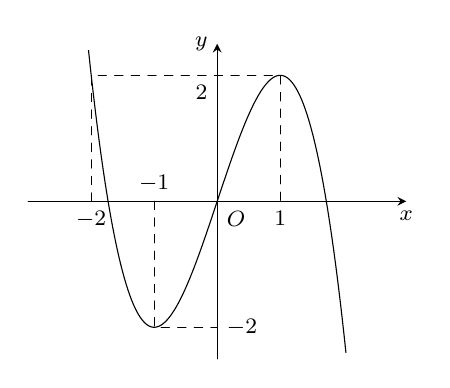
\begin{tikzpicture}[scale=.8,>=stealth,font=\footnotesize,line join=round,line cap=round]
			\def\a{-1} \def\b{0} \def\c{3} \def\d{0} 
			\def\xmin{-3} \def\xmax{3} 
			\def\ymin{-2.5} \def\ymax{2.5} 
			\draw[->]  (\xmin,0)--(\xmax,0) node [below]{$x$};
			\draw[->] (0,\ymin)--(0,\ymax) node [left]{$y$}; 
			\node at (0,0) [below right]{$O$}; 
			\clip (\xmin+0.1,\ymin+0.1) rectangle (\xmax-0.1,\ymax-0.1); 
			\draw[smooth,samples=300] plot (\x,{\a*(\x)^3+\b*(\x)^2+\c*(\x)+\d}); 
			\draw[dashed] (-2,0) node[below]{$-2$}--(-2,2)--(1,2)--(1,0)  node[below]{$1$}
				(-1,0) node[above]{$-1$}--(-1,-2)--(0,-2)  node[right]{$-2$}
				(0,2)  node[below left]{$2$};
		\end{tikzpicture}
	 }
	 \shortans{2014}
	 \loigiai{
		\centerline{ 
		$\begin{aligned}
		 &\ 9^{f(x)}+9m=m\cdot 3^{f(x)}+3^{f(x)+2} \\
		\Leftrightarrow  &\ 3^{2f(x)}-3^{f(x)+2}=m\left(3^{f(x)}-9\right)\\
		\Leftrightarrow &\ 3^{f(x)}\left( 3^{f(x)}-9 \right)=m\left( 3^{f(x)}-9 \right)\\ 
		\Leftrightarrow &\ \left[\begin{aligned}
		& 3^{f(x)}=9 \\ 
		 & 3^{f(x)}=m \\
	\end{aligned} \right.\\
	\Leftrightarrow &\ \left[\begin{aligned}
	& f(x)=2  &(1) \\
	& f(x)=\log_3m &(2) \\ 
	\end{aligned} \right.\\
	(1) \Leftrightarrow f(x)=2 \Leftrightarrow &\ \left[\begin{aligned}
	& x=-2 \\ 
	& x=1.  \\
	\end{aligned} \right.
	\end{aligned}$
	}\\ 
	Để phương trình có  đúng ba nghiệm thực phân biệt
	$\Leftrightarrow (2)$ có đúng 1 nghiệm thực khác $-2$ và  $1$\\
	$$\Leftrightarrow \left[\begin{aligned}
	& 2<\log_3m  \\
	 & \log_3m<-2 \\
	\end{aligned} \right. \Leftrightarrow
	\left[\begin{aligned}
	& m>9  \\
	 & m<\dfrac{1}{9}. \\
	\end{aligned} \right.$$
	Với  $m$ nguyên dương và nhỏ hơn $2024$ nên ta lấy
	$\left\{ \begin{aligned}
	& m\in \mathbb{Z} \\ 
	& 10\le m\le 2023.  \\
	\end{aligned} \right.$\\
	Vậy có $2014$ giá trị của tham  số $m$ thỏa mãn.
	} 
\end{ex}
